\documentclass[aspectratio=169,10pt]{beamer}

\usepackage[T1]{fontenc}
\usepackage[scaled=0.96]{helvet}
\usepackage{graphicx}
\usepackage{tikz}
\usepackage{xcolor}
\usepackage{array}

\renewcommand{\familydefault}{\sfdefault}
\graphicspath{{assets/}}

\definecolor{paper}{HTML}{F7F6F1}
\definecolor{ink}{HTML}{101820}
\definecolor{muted}{HTML}{586070}
\definecolor{line}{HTML}{D7D1C4}
\definecolor{teal}{HTML}{0B7A75}
\definecolor{blue}{HTML}{315C9A}
\definecolor{ochre}{HTML}{B86B2B}
\definecolor{plum}{HTML}{6D597A}

\setbeamertemplate{navigation symbols}{}
\setbeamertemplate{footline}{}
\setbeamercolor{background canvas}{bg=paper}
\setbeamercolor{normal text}{fg=ink}
\setbeamercolor{frametitle}{fg=ink}
\setbeamerfont{frametitle}{series=\bfseries,size=\Large}

\newcommand{\slidetitle}[1]{%
  \vspace*{0.15cm}
  {\Large\bfseries #1}\par
  \vspace{0.25cm}
}

\newcommand{\source}[1]{%
  \begin{tikzpicture}[remember picture,overlay]
    \node[anchor=south west, text=muted, font=\tiny] at ([xshift=0.46cm,yshift=0.22cm]current page.south west) {#1};
    \node[anchor=south east, text=muted, font=\tiny] at ([xshift=-0.46cm,yshift=0.22cm]current page.south east) {Giacomo Cappelletto \hspace{0.7em} \insertframenumber/\inserttotalframenumber};
  \end{tikzpicture}
}

\newcommand{\pill}[2][line]{%
  \tikz[baseline=(x.base)] \node[draw=#1, fill=white, rounded corners=2pt, inner xsep=5pt, inner ysep=3pt, font=\scriptsize\bfseries, text=ink] (x) {#2};
}

\newcommand{\bigword}[2]{%
  \begin{tikzpicture}
    \node[draw=#1, fill=white, rounded corners=3pt, line width=0.7pt, text width=3.0cm, minimum height=1.0cm, align=center, font=\bfseries] {#2};
  \end{tikzpicture}
}

\begin{document}

% Slide 1
\begin{frame}[plain]
  \begin{tikzpicture}[remember picture,overlay]
    \node[anchor=center, opacity=0.14] at (current page.center) {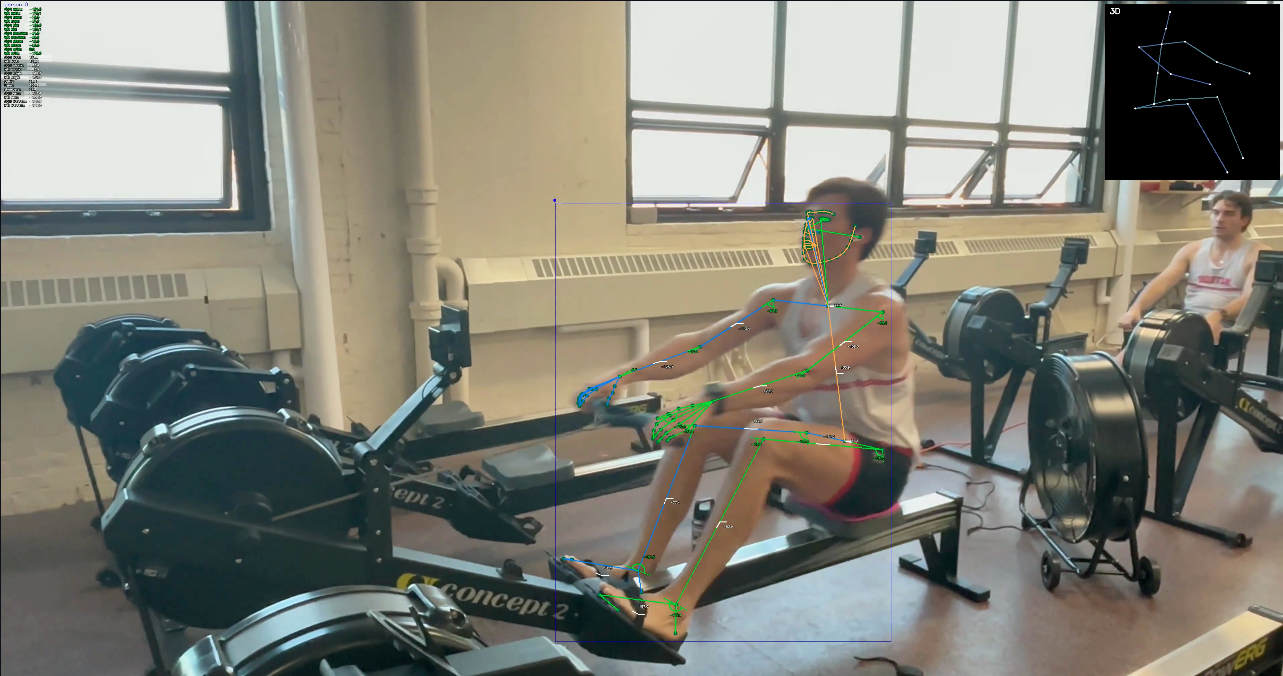
\includegraphics[width=\paperwidth]{rowing_pose_overlay.png}};
    \fill[paper, opacity=0.84] (current page.south west) rectangle (current page.north east);
    \node[anchor=west, text=ink, font=\bfseries\fontsize{28}{32}\selectfont] at ([xshift=0.85cm,yshift=0.70cm]current page.west) {Giacomo Cappelletto};
    \node[anchor=west, text=muted, font=\fontsize{13}{17}\selectfont] at ([xshift=0.88cm,yshift=-0.05cm]current page.west) {BU Computer Engineering \hspace{0.35em} | \hspace{0.35em} applied ML/CV \hspace{0.35em} | \hspace{0.35em} rowing biomechanics};
    \draw[teal, line width=1.2pt] ([xshift=0.88cm,yshift=-0.52cm]current page.west) -- ++(5.4cm,0);
    \node[anchor=west, text=ink, font=\fontsize{10}{13}\selectfont] at ([xshift=0.9cm,yshift=-1.02cm]current page.west) {Research opportunity conversation with Prof. Wei-Lun (Harry) Chao};
    \node[anchor=west, text=muted, font=\fontsize{8}{10}\selectfont] at ([xshift=0.9cm,yshift=-1.45cm]current page.west) {July 7, 2026};
  \end{tikzpicture}
  \note{Introduce yourself in under 20 seconds: BU computer engineering, rowing athlete, most recent research is video-derived rowing biomechanics and force-curve prediction.}
\end{frame}

% Slide 2
\begin{frame}[plain]
  \slidetitle{How I got into AI/ML}
  \vspace{0.4cm}
  \begin{tikzpicture}[x=1cm,y=1cm]
    \draw[line, line width=1.1pt] (0.6,1.9) -- (11.7,1.9);

    \foreach \x/\c/\t/\s in {
      0.9/teal/{age 15}/{agents + RAG},
      3.2/blue/{2024}/{MNIST in NumPy},
      5.5/ochre/{2024}/{CIFAR-10 NAS},
      7.8/plum/{2025}/{OCR to LaTeX/PDF},
      10.3/teal/{2026}/{video to force curves}
    } {
      \fill[\c] (\x,1.9) circle (3.8pt);
      \node[anchor=south, text=\c, font=\scriptsize\bfseries] at (\x,2.18) {\t};
      \node[anchor=north, text=ink, align=center, font=\scriptsize\bfseries, text width=1.75cm] at (\x,1.55) {\s};
    }

    \node[draw=line, fill=white, rounded corners=3pt, inner sep=3pt] at (3.2,0.35) {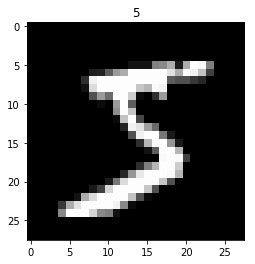
\includegraphics[width=2.0cm]{mnist.png}};
    \node[draw=line, fill=white, rounded corners=3pt, inner sep=6pt] at (5.5,0.35) {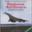
\includegraphics[width=0.85cm,interpolate=false]{cifar_sample.png}};
    \node[draw=line, fill=white, rounded corners=3pt, inner sep=3pt] at (10.3,0.35) {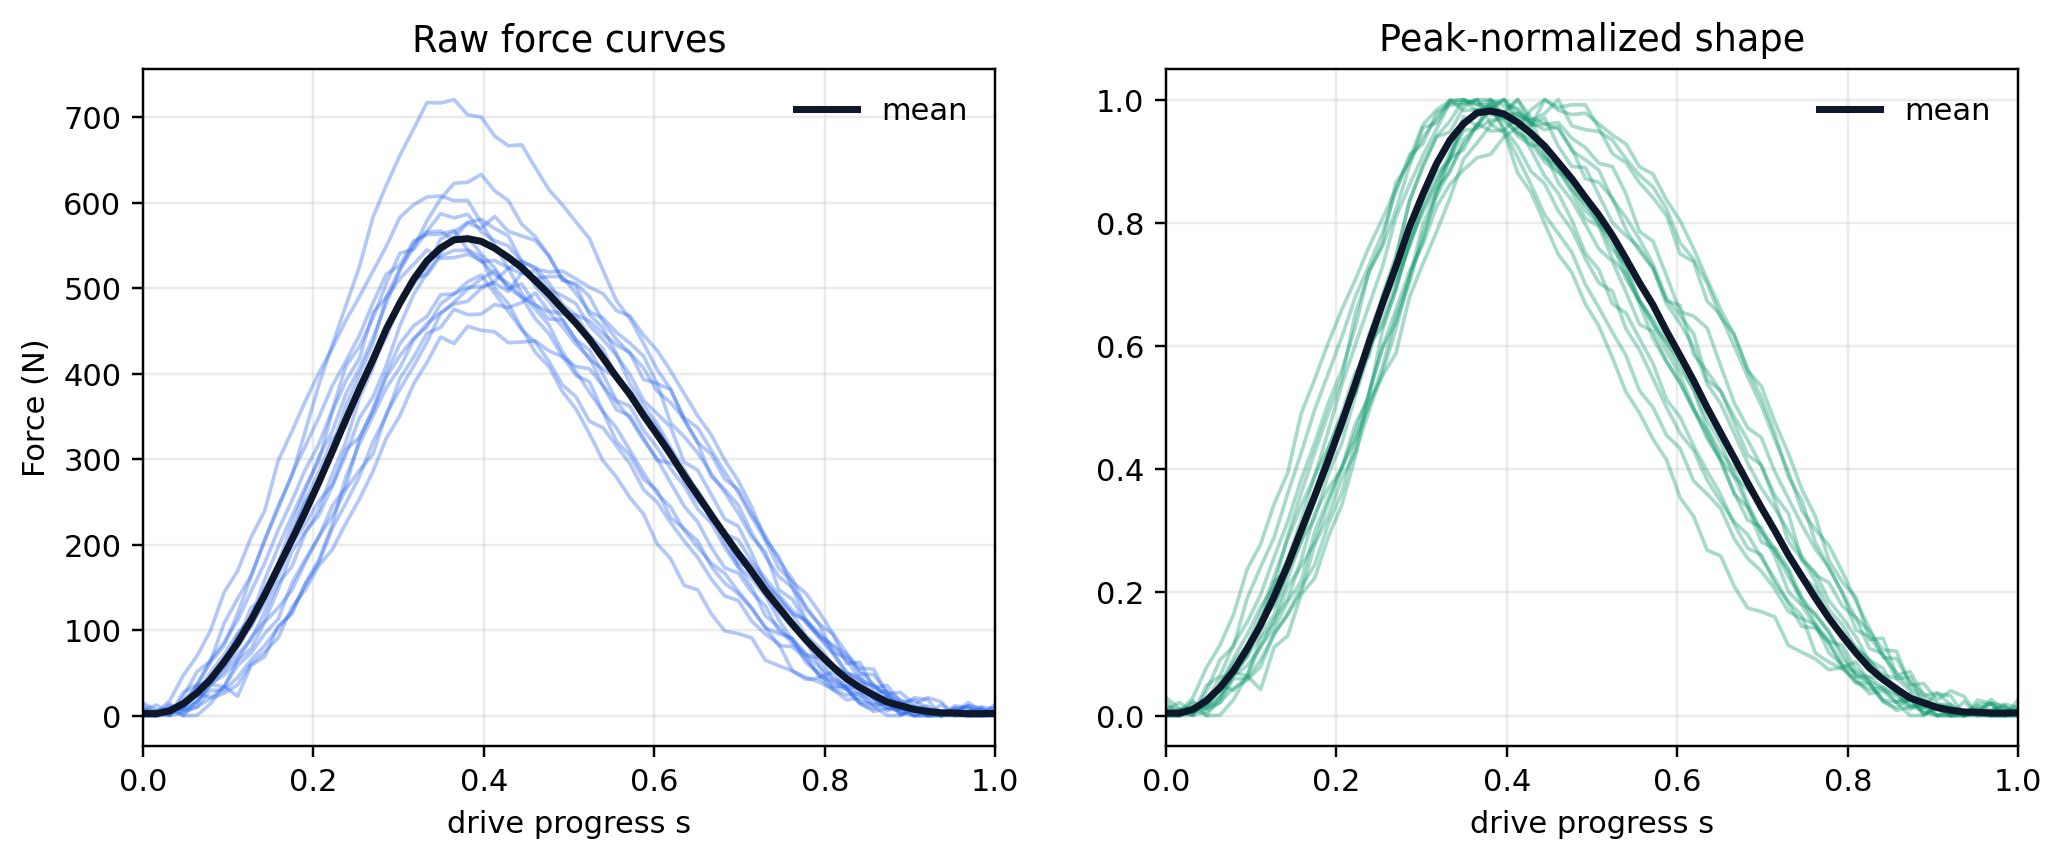
\includegraphics[width=2.05cm]{rowing_force_curves.png}};
  \end{tikzpicture}

  \vspace{0.6cm}
  \begin{center}
    {\Large\bfseries Now: computer vision, deep learning, and real-world signals}
  \end{center}
  \note{Say: I started by building useful AI tools, then basic neural networks, then image recognition/NAS, then OCR and document generation, and the latest project made me care about rigorous CV and sequence modeling.}
\end{frame}

% Slide 3
\begin{frame}[plain]
  \slidetitle{Latest research: video-to-force inference}
  \begin{columns}[T,totalwidth=\textwidth]
    \begin{column}{0.50\textwidth}
      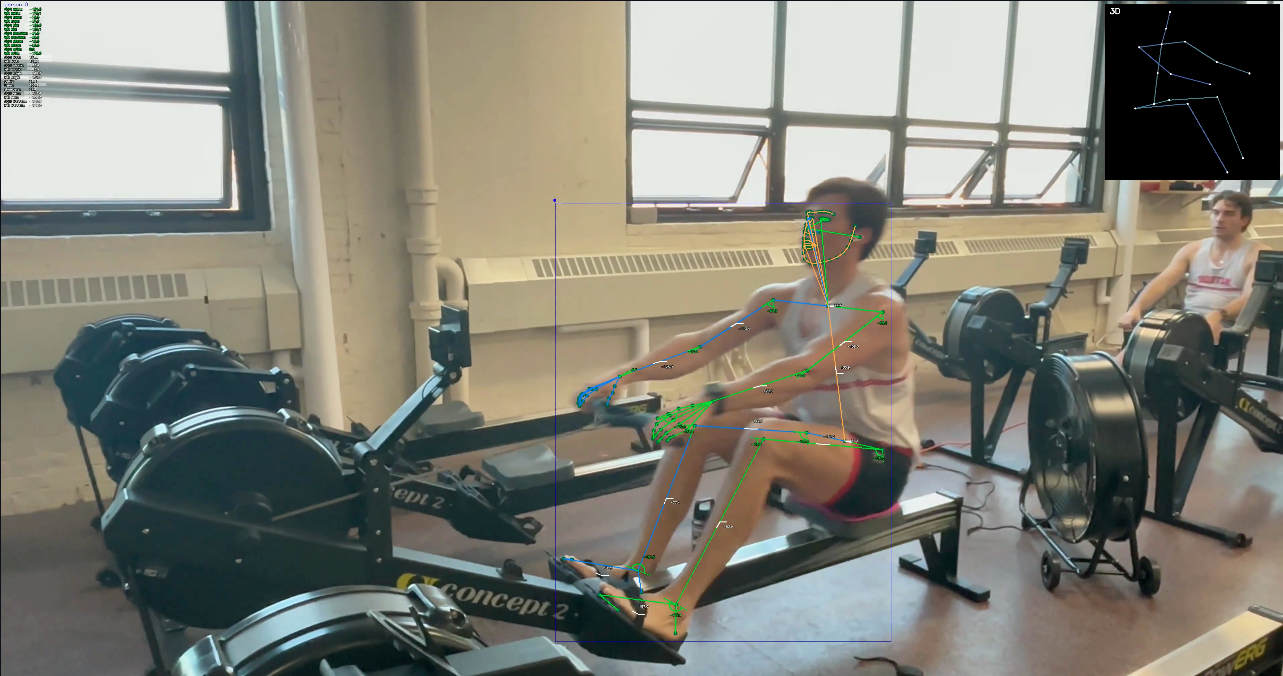
\includegraphics[width=\linewidth,trim=0 22 0 0,clip]{rowing_pose_overlay.png}
      \vspace{0.15cm}
      \centering{\scriptsize\bfseries Video -> pose / kinematics}
    \end{column}
    \begin{column}{0.48\textwidth}
      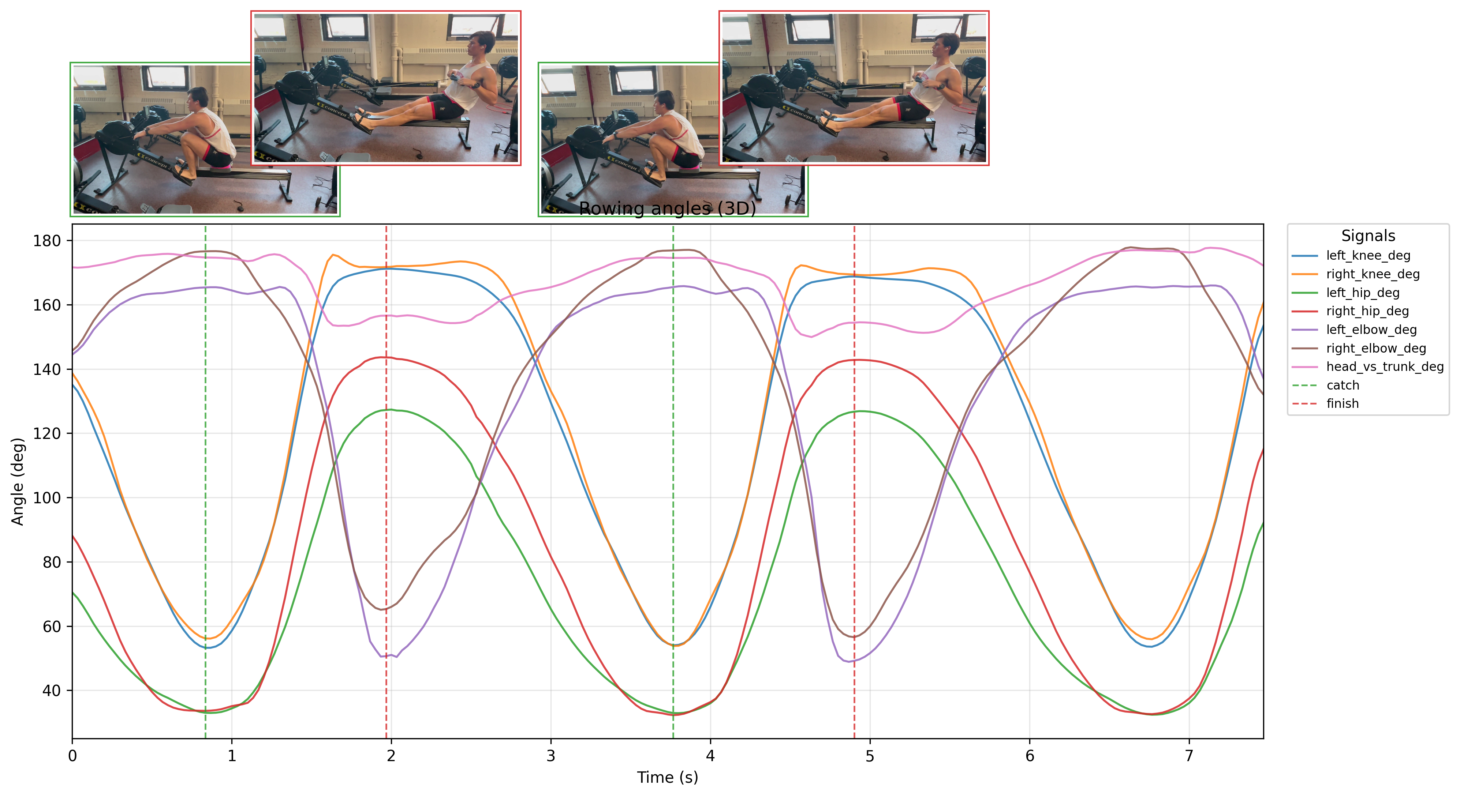
\includegraphics[width=\linewidth]{side-graph-s2d.png}
      \vspace{0.15cm}
      \centering{\scriptsize\bfseries RP3 force curves -> sequence targets}
    \end{column}
  \end{columns}

  \vspace{0.35cm}
  \begin{center}
    \pill[teal]{Sports2D / MotionBERT}
    \hspace{0.35cm}
    \pill[blue]{drive-progress alignment}
    \hspace{0.35cm}
    \pill[ochre]{TCN / Transformer}
  \end{center}
  \note{Keep it short: goal was to test whether phone-quality video can predict rowing force curves. Emphasize your role: data collection, pose tracking, sync/alignment, normalization, early sequence modeling.}
\end{frame}

% Slide 4
\begin{frame}[plain]
  \begin{tikzpicture}[remember picture,overlay]
    \node[anchor=center, opacity=0.16] at (current page.center) {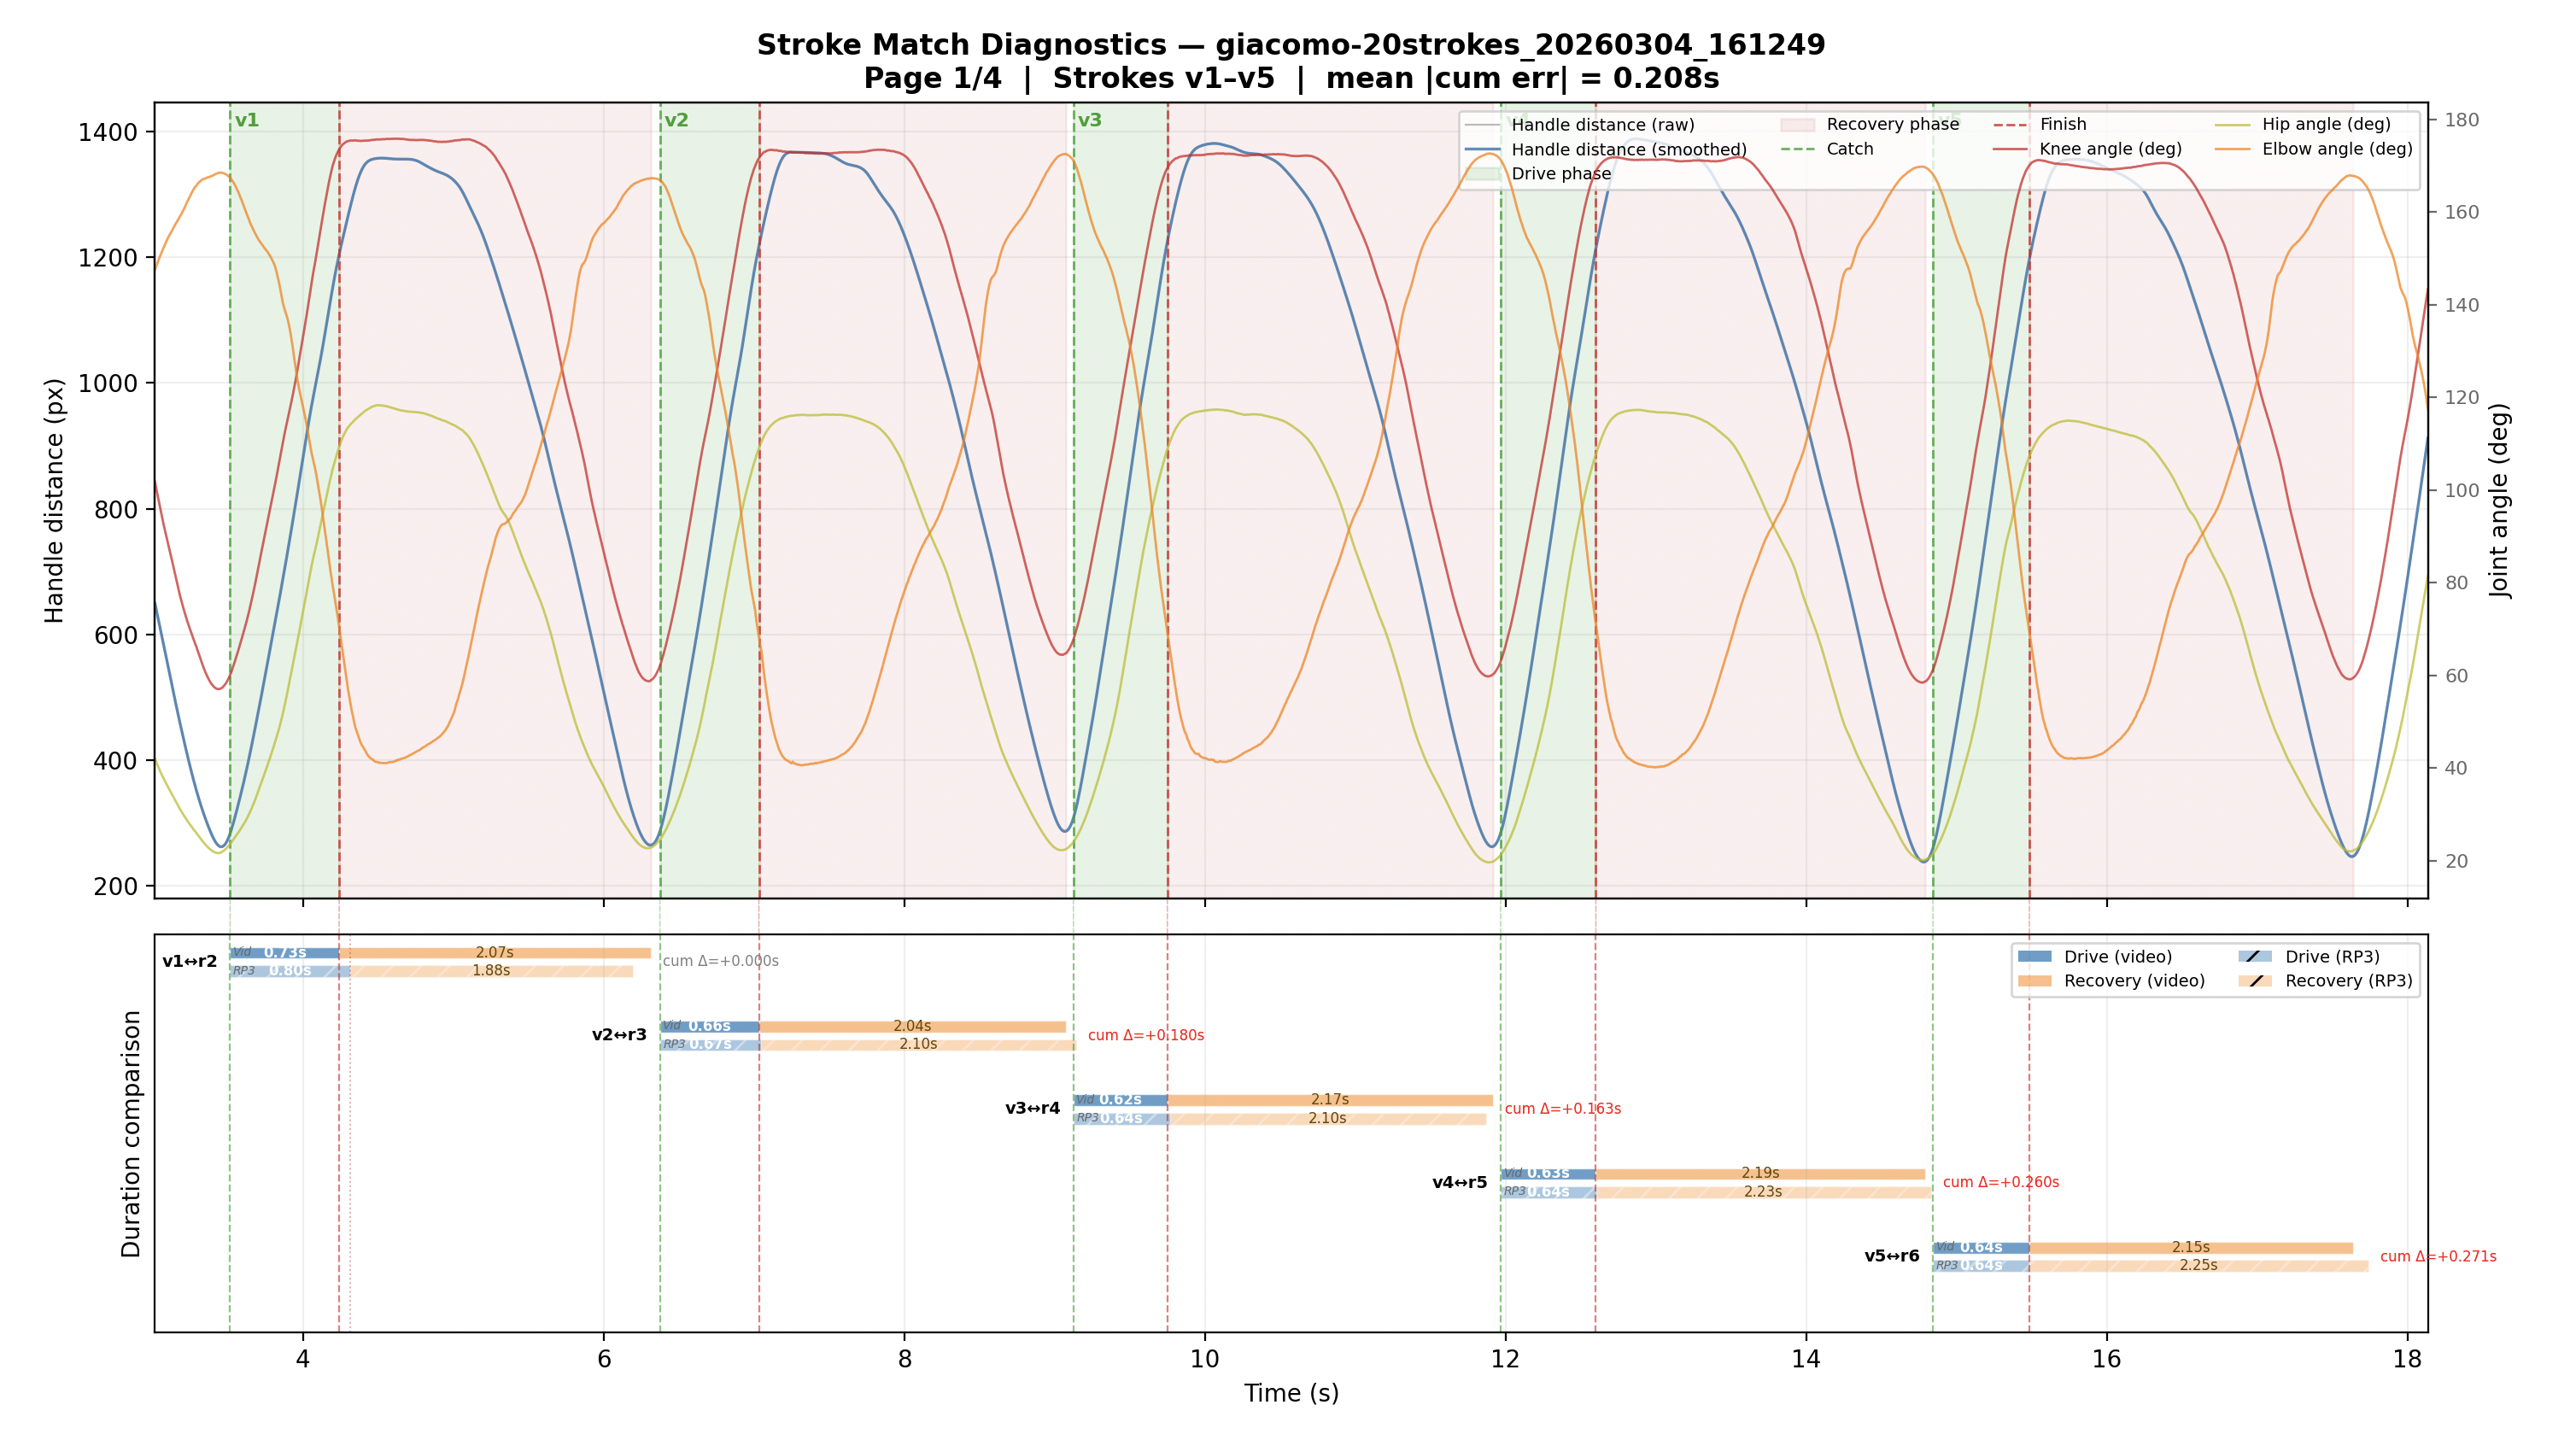
\includegraphics[width=1.05\paperwidth]{rowing_matching_diagnostic.png}};
    \fill[paper, opacity=0.82] (current page.south west) rectangle (current page.north east);
  \end{tikzpicture}

  \vspace*{1.0cm}
  \begin{center}
    {\fontsize{25}{31}\selectfont\bfseries The hard part was not the model.}

    \vspace{0.8cm}
    \bigword{teal}{alignment}
    \hspace{0.6cm}
    \bigword{blue}{quality control}
    \hspace{0.6cm}
    \bigword{ochre}{generalization}

    \vspace{0.75cm}
    {\large limited paired data + occlusion + drift}
  \end{center}
  \note{This is the main research maturity slide. Say that the bottleneck became data structure and validation: pose errors, synchronization, and label drift shaped the research more than picking a bigger model.}
\end{frame}

% Slide 5
\begin{frame}[plain]
  \slidetitle{Why this opportunity fits}
  \vspace{0.2cm}
  \begin{columns}[T,totalwidth=\textwidth]
    \begin{column}{0.46\textwidth}
      {\small\bfseries Your group's themes}

      \vspace{0.35cm}
      \pill[teal]{imperfect data}\quad
      \pill[teal]{robust perception}

      \vspace{0.22cm}
      \pill[blue]{multi-source data}\quad
      \pill[blue]{transfer}

      \vspace{0.22cm}
      \pill[ochre]{domain adaptation}\quad
      \pill[ochre]{vision-language}
    \end{column}

    \begin{column}{0.48\textwidth}
      {\small\bfseries What I want to grow into}

      \vspace{0.35cm}
      \pill[plum]{computer vision}\quad
      \pill[plum]{deep learning}

      \vspace{0.22cm}
      \pill[teal]{sequence models}\quad
      \pill[teal]{evaluation}

      \vspace{0.22cm}
      \pill[blue]{real-world noisy data}\quad
      \pill[blue]{research rigor}
    \end{column}
  \end{columns}

  \vfill
  \note{Mention that your project is not the same domain as autonomous driving or Imageomics, but it hits similar methodological issues: noisy perception, limited labels, alignment, and evaluation.}
\end{frame}

% Slide 6
\begin{frame}[plain]
  \slidetitle{What I hope to do}
  \vspace{0.15cm}
  \begin{columns}[T,totalwidth=\textwidth]
    \begin{column}{0.31\textwidth}
      {\small\bfseries Contribute}
      \vspace{0.25cm}

      \pill[teal]{Python ML pipelines}

      \vspace{0.2cm}
      \pill[teal]{data cleaning / QC}

      \vspace{0.2cm}
      \pill[teal]{reproducible experiments}
    \end{column}
    \begin{column}{0.31\textwidth}
      {\small\bfseries Learn}
      \vspace{0.25cm}

      \pill[blue]{research design}

      \vspace{0.2cm}
      \pill[blue]{CV / deep learning depth}

      \vspace{0.2cm}
      \pill[blue]{evaluation discipline}
    \end{column}
    \begin{column}{0.31\textwidth}
      {\small\bfseries Availability}
      \vspace{0.25cm}

      \pill[ochre]{AU26: 10-15 h/wk}

      \vspace{0.2cm}
      \pill[ochre]{SP27: ~10 h/wk}

      \vspace{0.2cm}
      \pill[ochre]{Aug: light remote prep}
    \end{column}
  \end{columns}
  \note{End by saying: I want more research experience and a better understanding of how strong research questions become experiments and papers.}
\end{frame}

\end{document}
